\section{Durchführung}
\label{sec:Durchführung}
    \begin{figure}
      \centering
      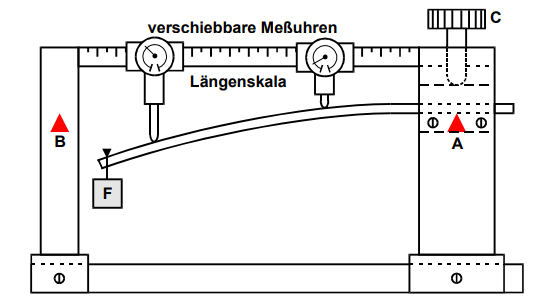
\includegraphics{content/apparatur.png}
      \caption{Aufbau einer Apparatur zur Bestimmung der Durchbiegung elastischer Stäbe \cite[111]{V103}}
      \label{fig:apparatur}
    \end{figure}
    Die Biegung verschiedener elastischer Stäbe wird mit der Apparatur, welche in \autoref{fig:apparatur} zu sehen ist, gemessen.
    Insgesamt werden hiermit die Durchbiegungen dreier Stäbe bestimmt; von einem eckigen und einem runden Stab durch einseitige Einspannung
    und einem eckigen Stab durch beidseitige Einhängung. Von allen Stäben werden die geometrischen Eigenschaften bestimmt.
    Das Gewicht der anzuhängenden Gewichte ist ebenfalls zu bestimmen.


    Bei der einseitigen Einspannung wird der Stab an der Vorrichtung C aus \autoref{fig:apparatur} eingespannt. Anschließend wird eine Nullmessung 
    an dem Stab durchgeführt, das heißt der Stab wird zunächst ohne angehängtes Gewicht mittels einer Messuhr vermessen; anschließend
    wird die Messung mit angehängtem Gewicht wiederholt. Die einzelnen Messchritte haben in der Nähe der Einspannung einen Abstand von
    3cm und sonst einen Abstand von 2cm. Insgesamt werden so 22 Messungen je Stab durchgeführt.


    Bei der beidseitigen Einspannung liegt der Stab zusätlich an der Befestigung B aus \autoref{fig:apparatur} auf. Nun werden beide Messuhren verwendet
    um zunächst wieder eine Nullmessung durchzuführen, wobei jeweils nur bis zur Mitte des Stabes gemessen werden darf. 
    Danach wird in die Mitte des Stabes ein Gewicht gehängt und die Messuhren messen wieder zur Mitte hin die Durchbiegung auf
    beiden Stabhälften. Die Abstände der Messpunkt sind die gleichen, wie bei der einseitigen Einspannung auch, nur dass beachtet
    werden muss, dass von beiden Seiten gemessen wird.